% This paper was written on overleaf.com or whatever website and pretty convinient

\documentclass{article}
\usepackage{graphicx} % Required for inserting images
\usepackage{subcaption}
\usepackage[top=1.2in, bottom=1.2in]{geometry}
\usepackage{fourier}
\usepackage{float}
\usepackage{amsmath}


\DeclareMathAlphabet{\mathcal}{OMS}{cmsy}{m}{n}
\SetMathAlphabet{\mathcal}{bold}{OMS}{cmsy}{b}{n}

\title{Eclipse-10000}
\author{Qclipsing}
\date{July 2026}
\raggedbottom

\begin{document}

\maketitle

\section{Introduction}
In this project, I have successfully recreated a full computer stack from scratch, starting with designing a 16-bit CPU in Logisim-Evolution using only logic gates and low-level components - such as splitters, bit extenders, pins, RAM, and ROM - with a custom ISA. 
Afterward, I created a separate 32-bit CPU using the SystemVerilog hardware description language, also featuring a custom ISA. 
Following that, I built my own compiler that translates my custom programming language into assembly, which then assembles into machine code instructions for that 32-bit CPU. My next step is developing an operating system for this CPU in my language.


\section{Eclipse-10000}
The whole project is named after this CPU I initially designed in Logisim, so let us start from it. It is a 16-bit multi-cycle CPU with a custom ISA (\texttt{ISA16.txt} file); I have built a simple 2-pass assembler for it.

\begin{figure}[H]
    \centering
    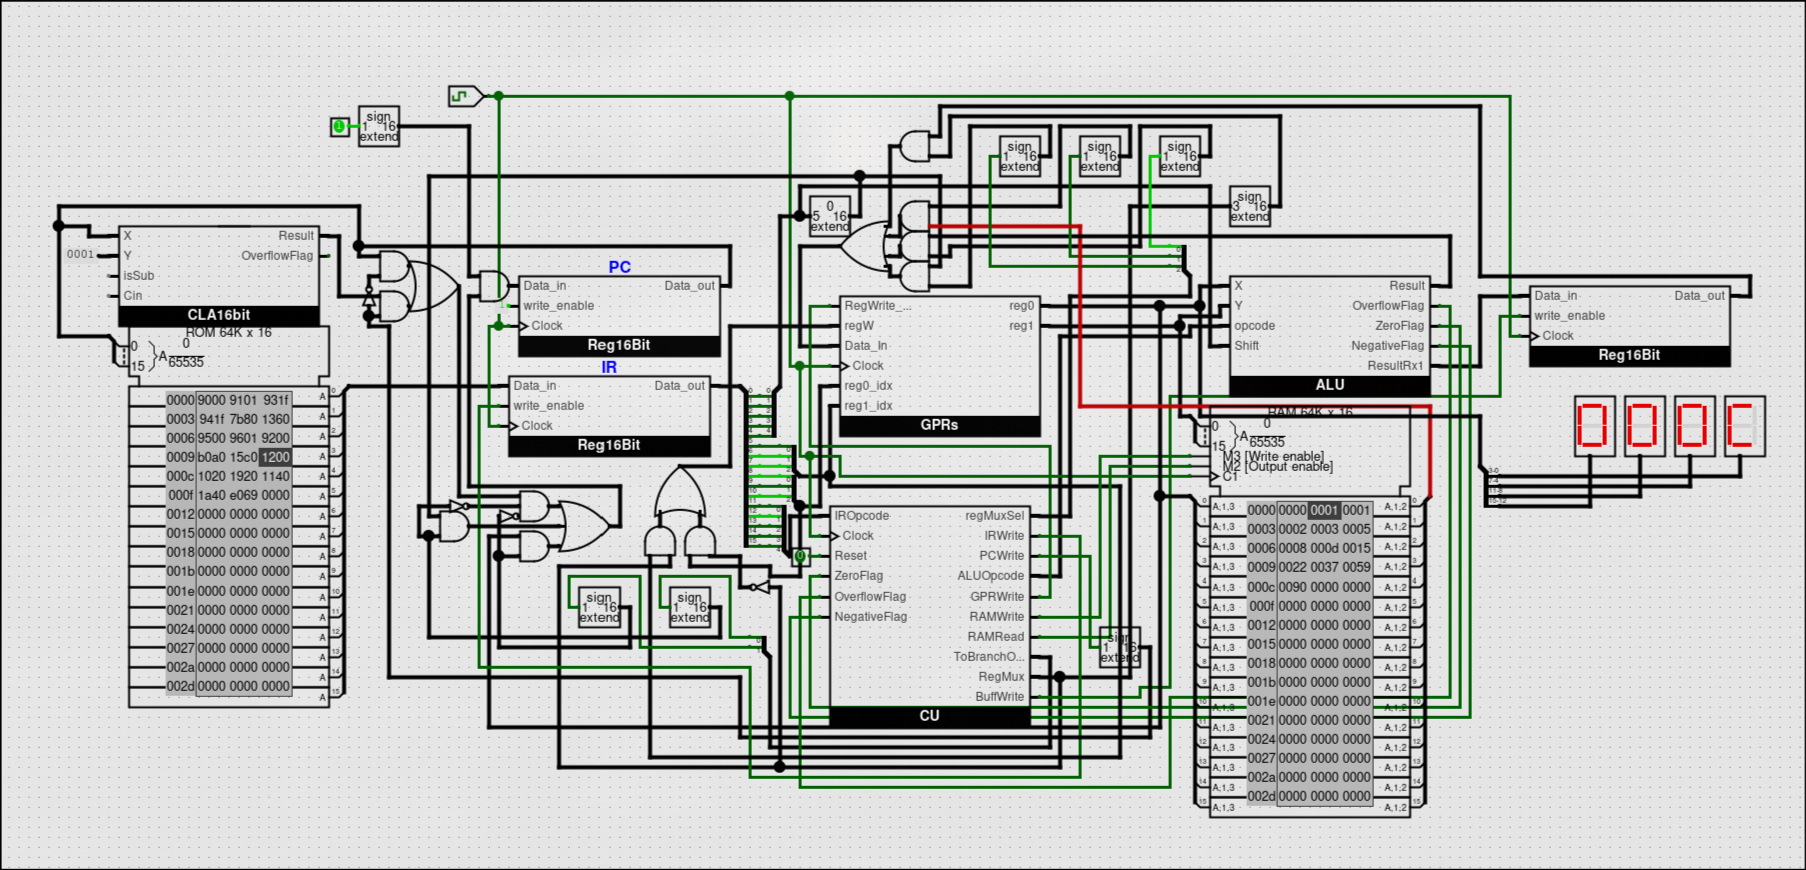
\includegraphics[width=0.7\textwidth]{Core.png}
    \caption{Diagram of the Core module calculating Fibonacci numbers}
    \label{fig:cpu_core}
\end{figure}

\subsection{ALU}
The ALU (Arithmetic Logic Unit) is one of the main CPU parts, so I gave it a lot of attention. It includes: AddSub module, Bitwise: AND, XOR, OR, NOT, SHL, SHR, and multiplication modules. It has a 4-to-16 bit decoder at its core. It also calculates all necessary flags: negative, overflow, and zero flags. 

\begin{figure}[H]
    \centering
    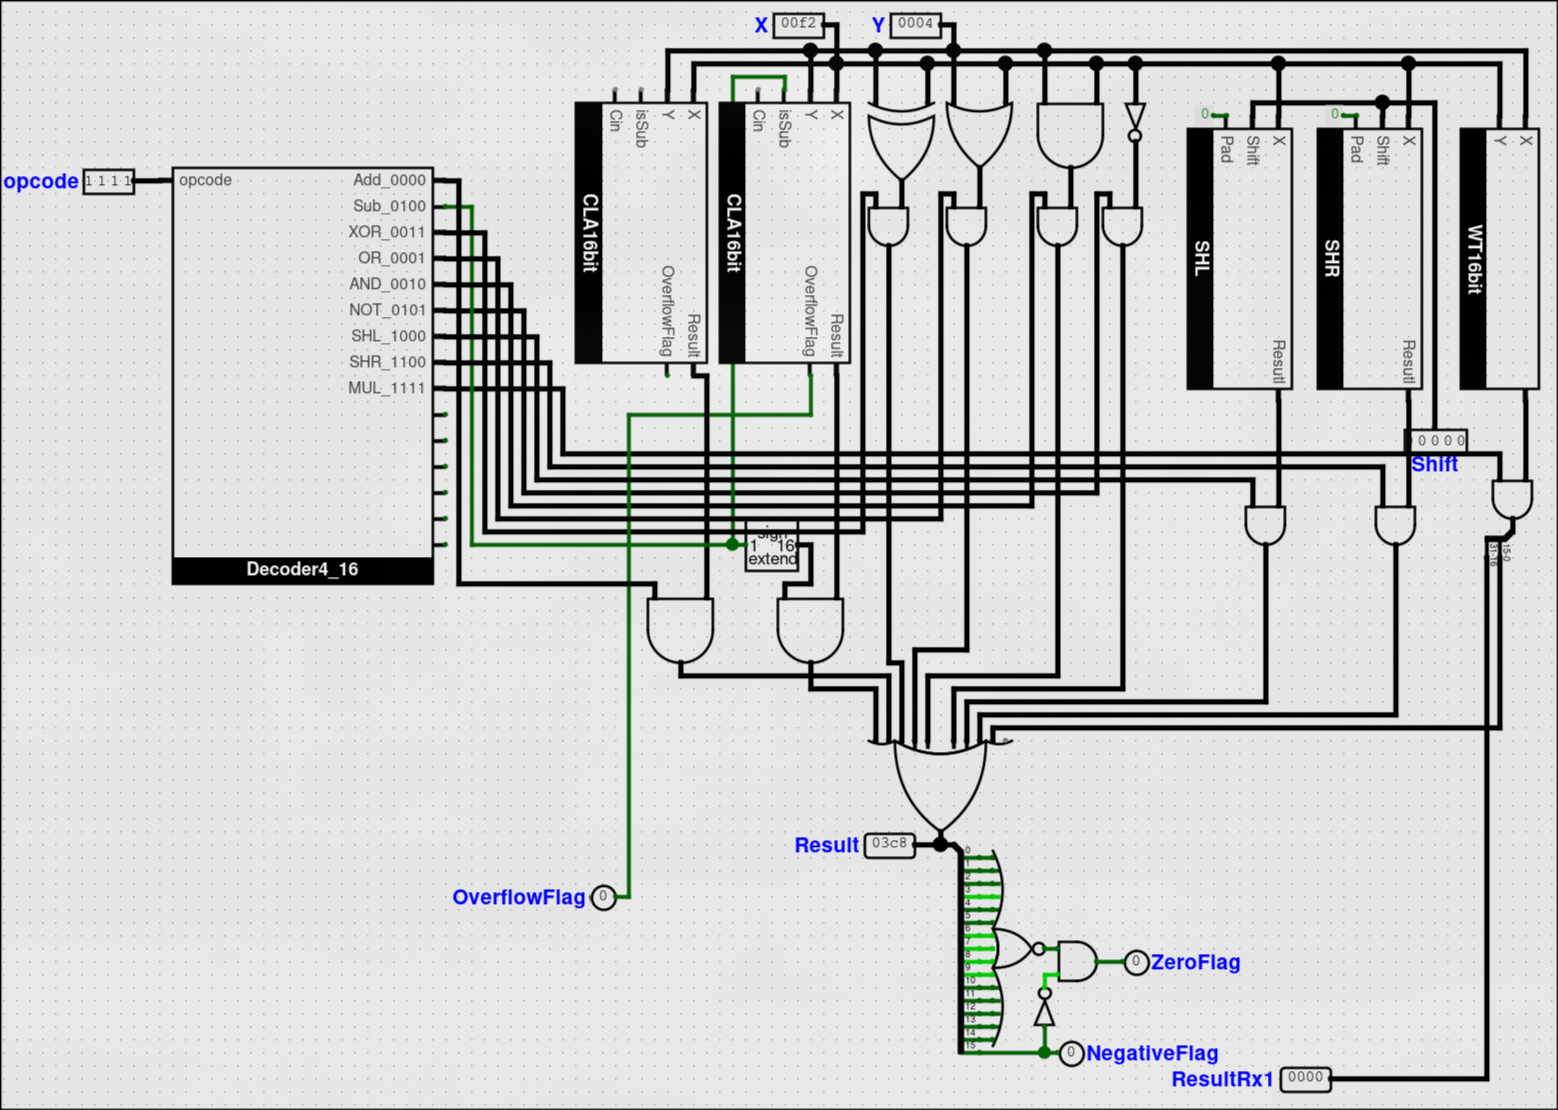
\includegraphics[width=0.55\textwidth]{ALU.png}
    \caption{Diagram of the ALU module performing 0x00f2 * 0x0004}
    \label{fig:alu_diagram}
\end{figure}

\subsubsection{16-bit CLA}
The CLA (Carry Lookahead Adder) is an adder/subtractor pair. I split them into 4 smaller 4-bit CLAs, each one emitting Propagation and Generation signals, and then wired them up in the main module as I would wire a basic 4-bit CLA. That reduced the complexity of the building process while maintaining speed.

\begin{figure}[H]
    \centering
    \begin{subfigure}[b]{0.48\textwidth}
        \centering
        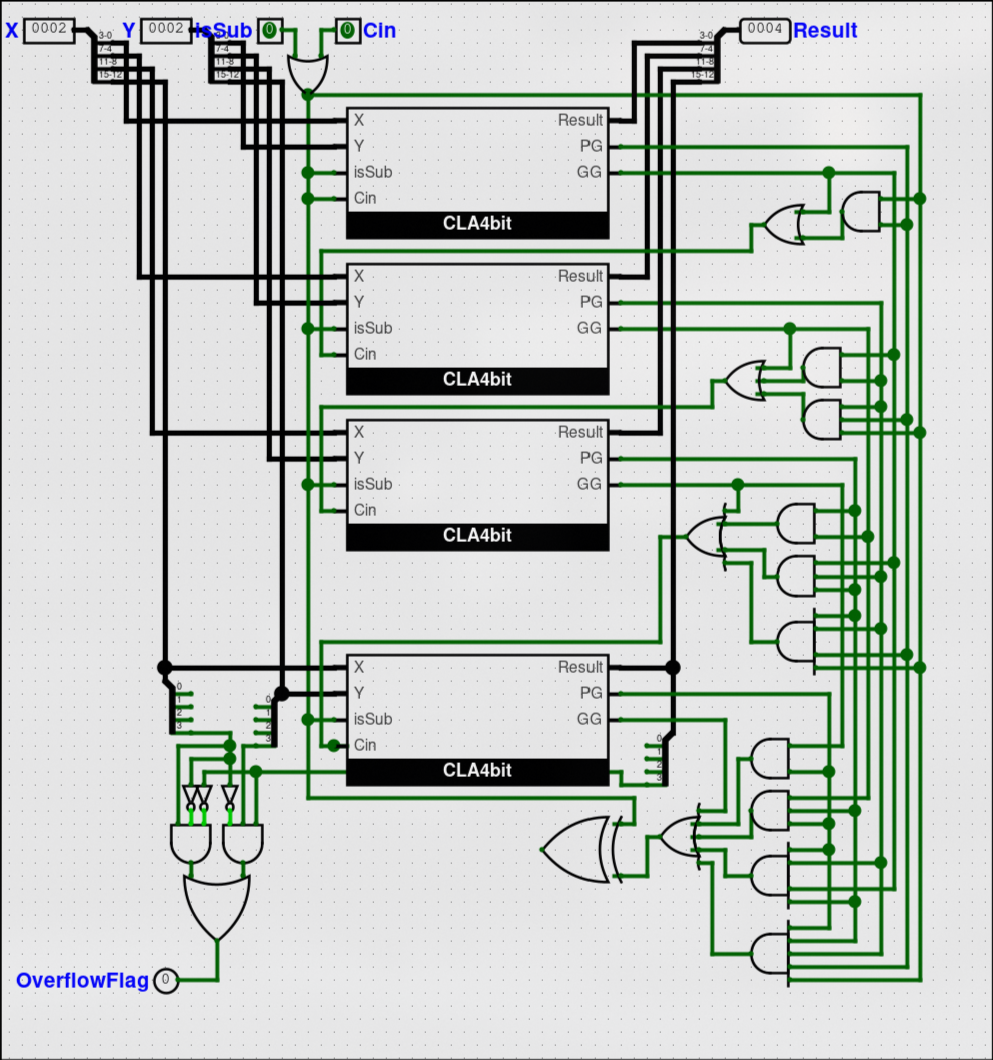
\includegraphics[width=\textwidth]{CLA16.png}
        \caption{Full 16-bit CLA}
        \label{fig:cla16}
    \end{subfigure}
    \hfill
    \begin{subfigure}[b]{0.48\textwidth}
        \centering
        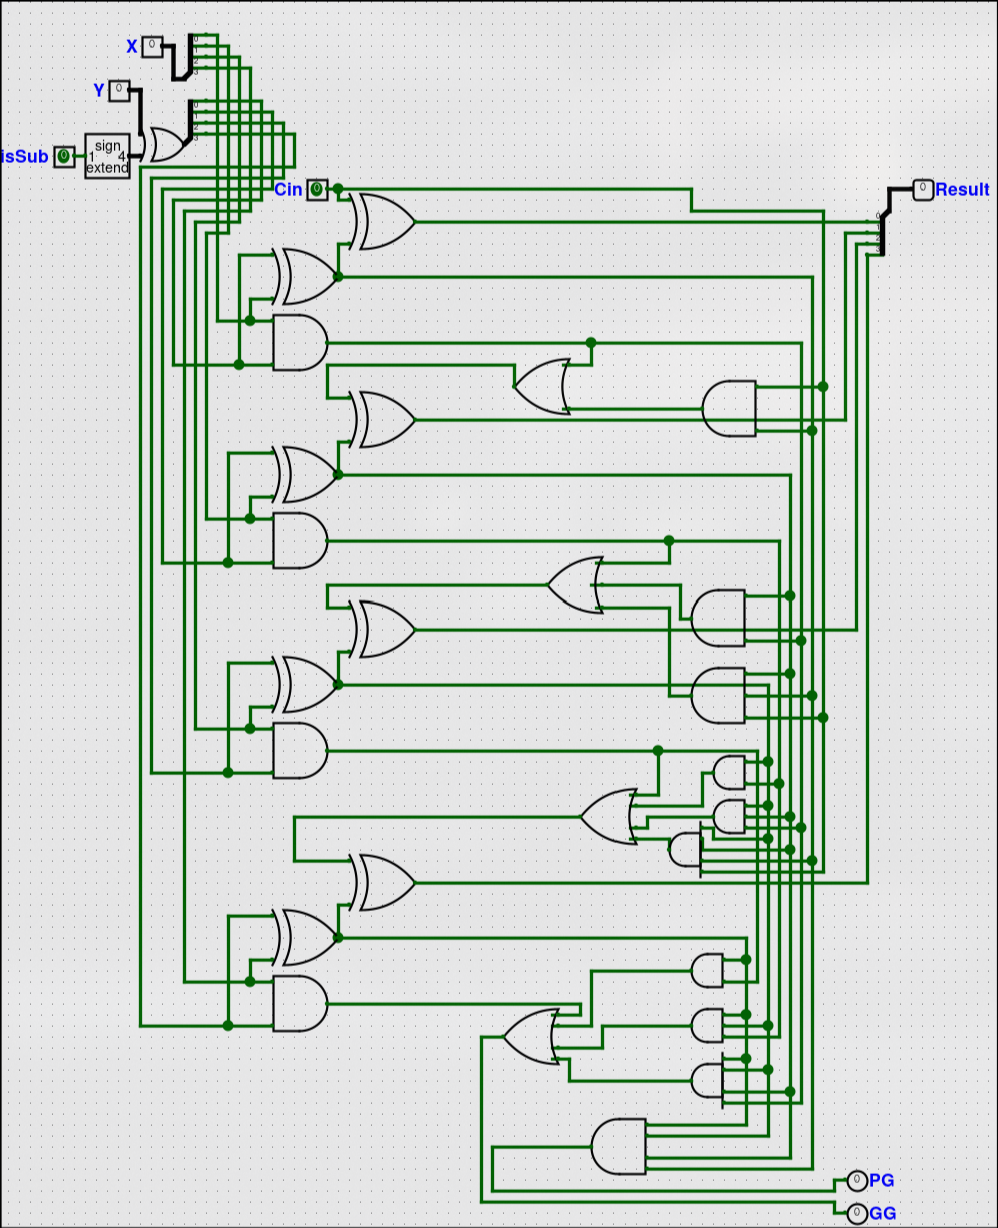
\includegraphics[width=\textwidth]{CLA4.png}
        \caption{Sub 4-bit CLA}
        \label{fig:cla4}
    \end{subfigure}
    \caption{4-bit CLA next to 16-bit CLA performing 2+2}
    \label{fig:cla_comparison}
\end{figure}

\subsubsection{16-bit Barrel Shifter and Bitwise Operations}
Standard bitwise operations (XOR, OR, AND, NOT) are performed using multi-bit input/output logic gates, whereas SHL and SHR are implemented using a barrel shifter in order to keep the shifting within 1 CPU cycle.

\begin{figure}[H]
    \centering
    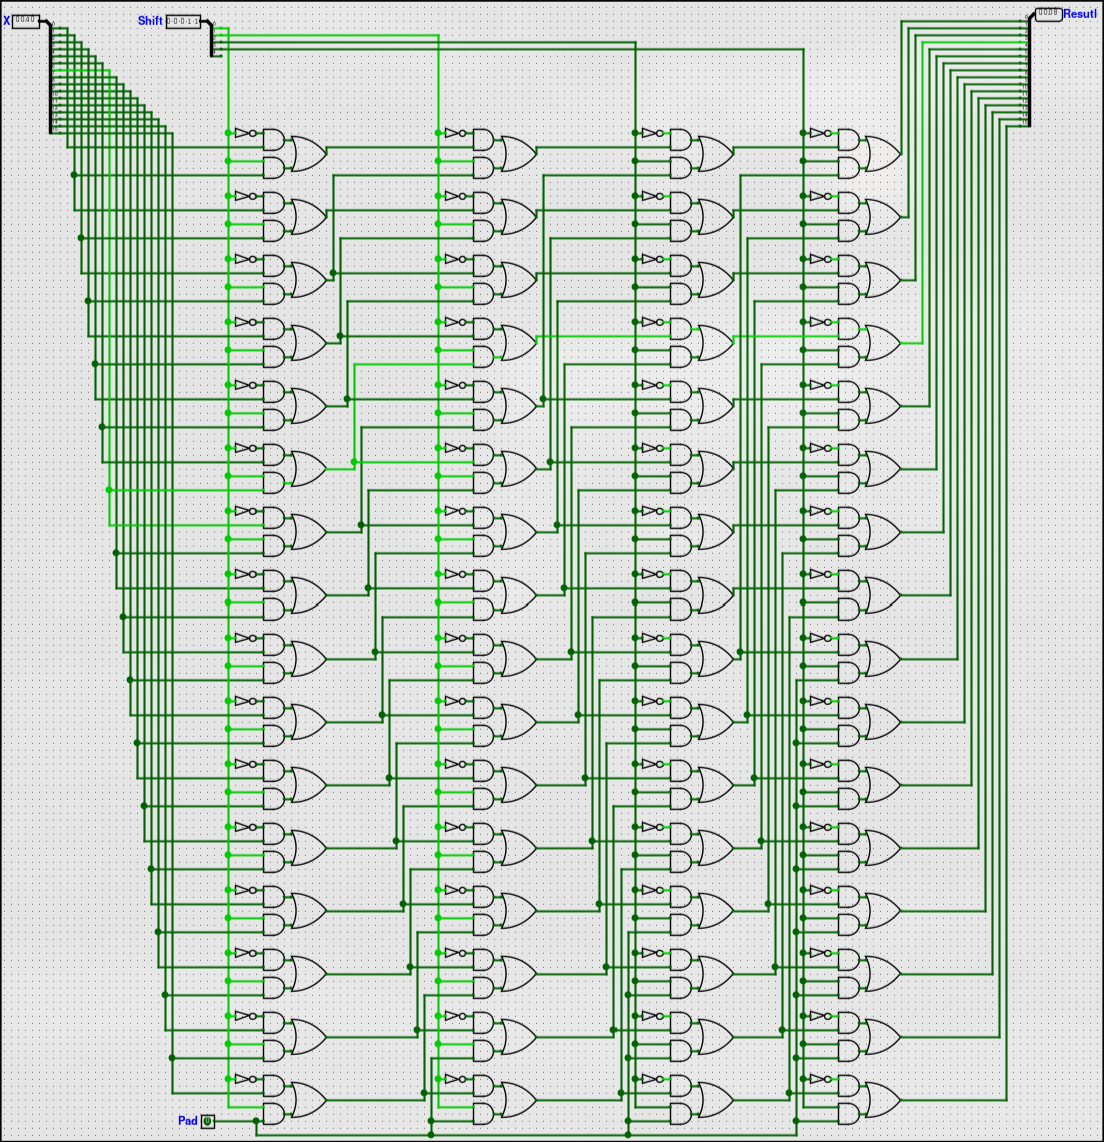
\includegraphics[width=0.55\textwidth]{Shifter16.png}
    \caption{Diagram of the 16-bit SHR, shifting 0x0040 right by 0b0011}
    \label{fig:shifter_diagram}
\end{figure}

\subsubsection{16-bit Wallace Tree}
The Wallace tree is the multiplier module of the ALU. It is a better version of a regular array multiplier due to its usage of full and half adders as 3:2 and 2:2 compressors, and its time complexity is $\mathcal{O}(\log n)$. I have used the same principle as in the CLA, separating it into 4-bit sub-modules and combining them. However, it was more challenging to implement; I had to shift result bits and pad them with zeros in order to make it work. 
Multiplication of two 16-bit variables can result in a value up to 32 bits long; I solved this by storing the lower 16 bits in the first operand and the higher 16 bits in the second operand. 

\begin{figure}[H]
    \centering
    \begin{subfigure}[b]{0.45\textwidth}
        \centering
        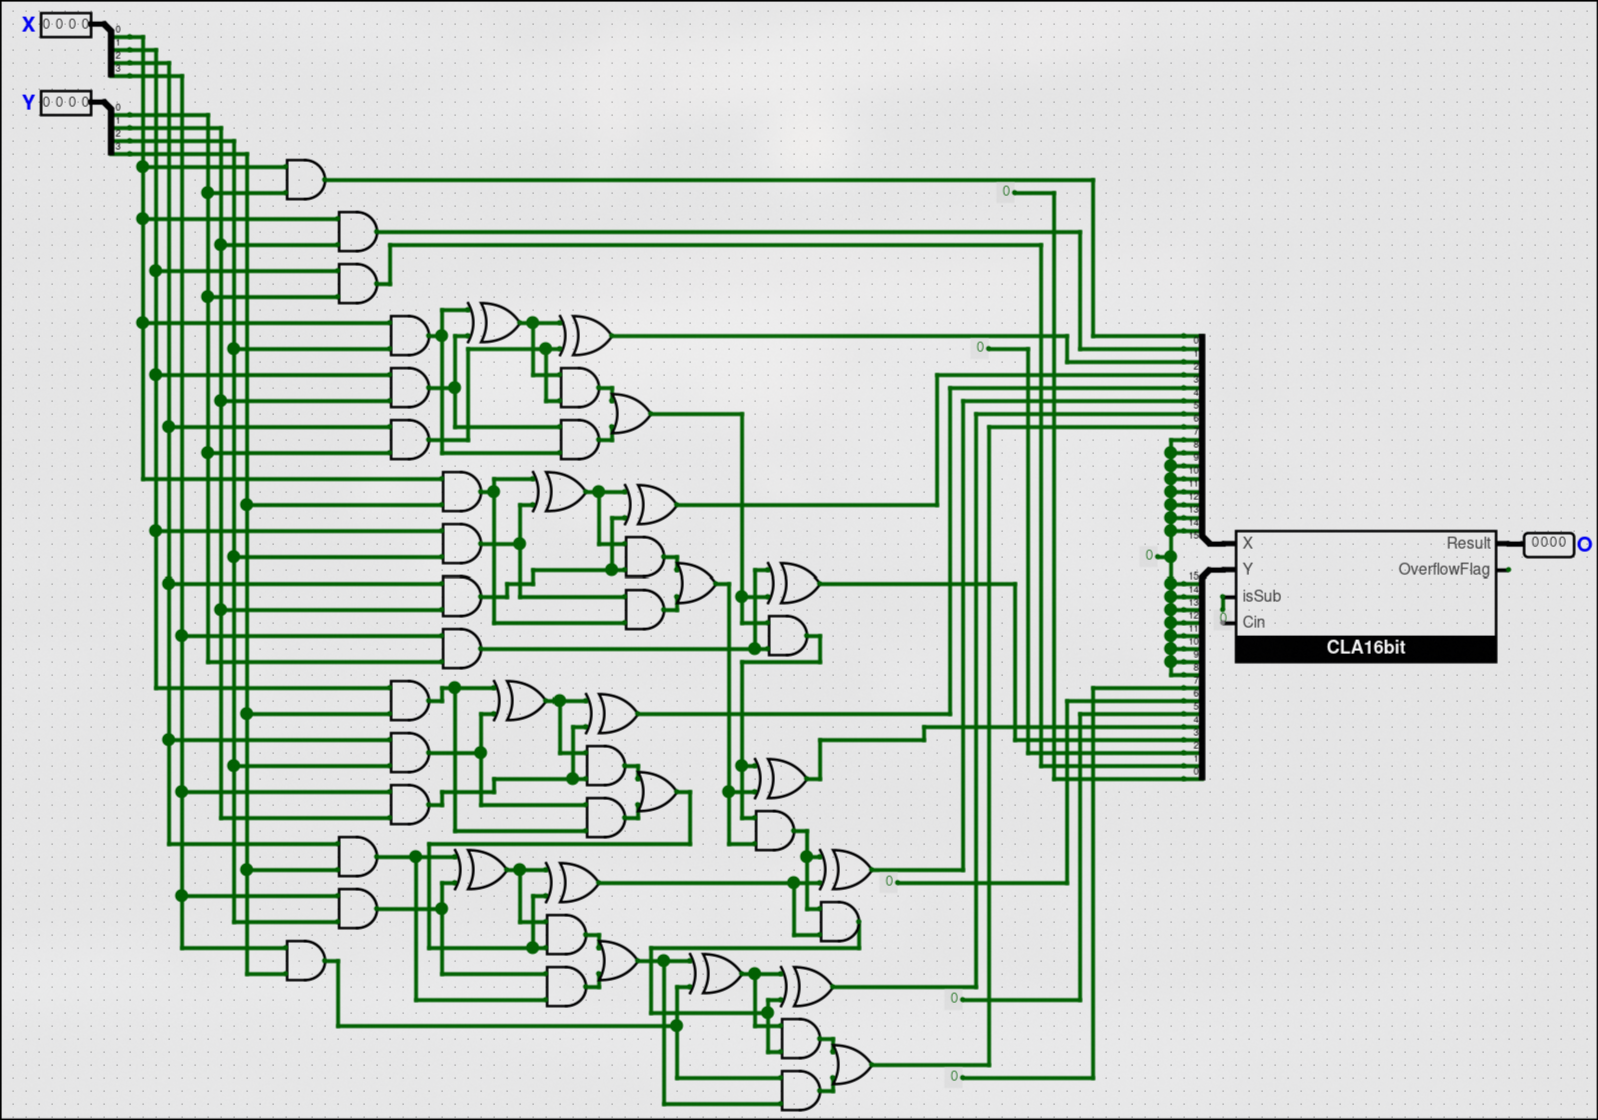
\includegraphics[width=\textwidth]{WT4.png}
        \caption{Small 4-bit Wallace Tree}
        \label{fig:wt4}
    \end{subfigure}
    \hfill
    \begin{subfigure}[b]{0.45\textwidth}
        \centering
        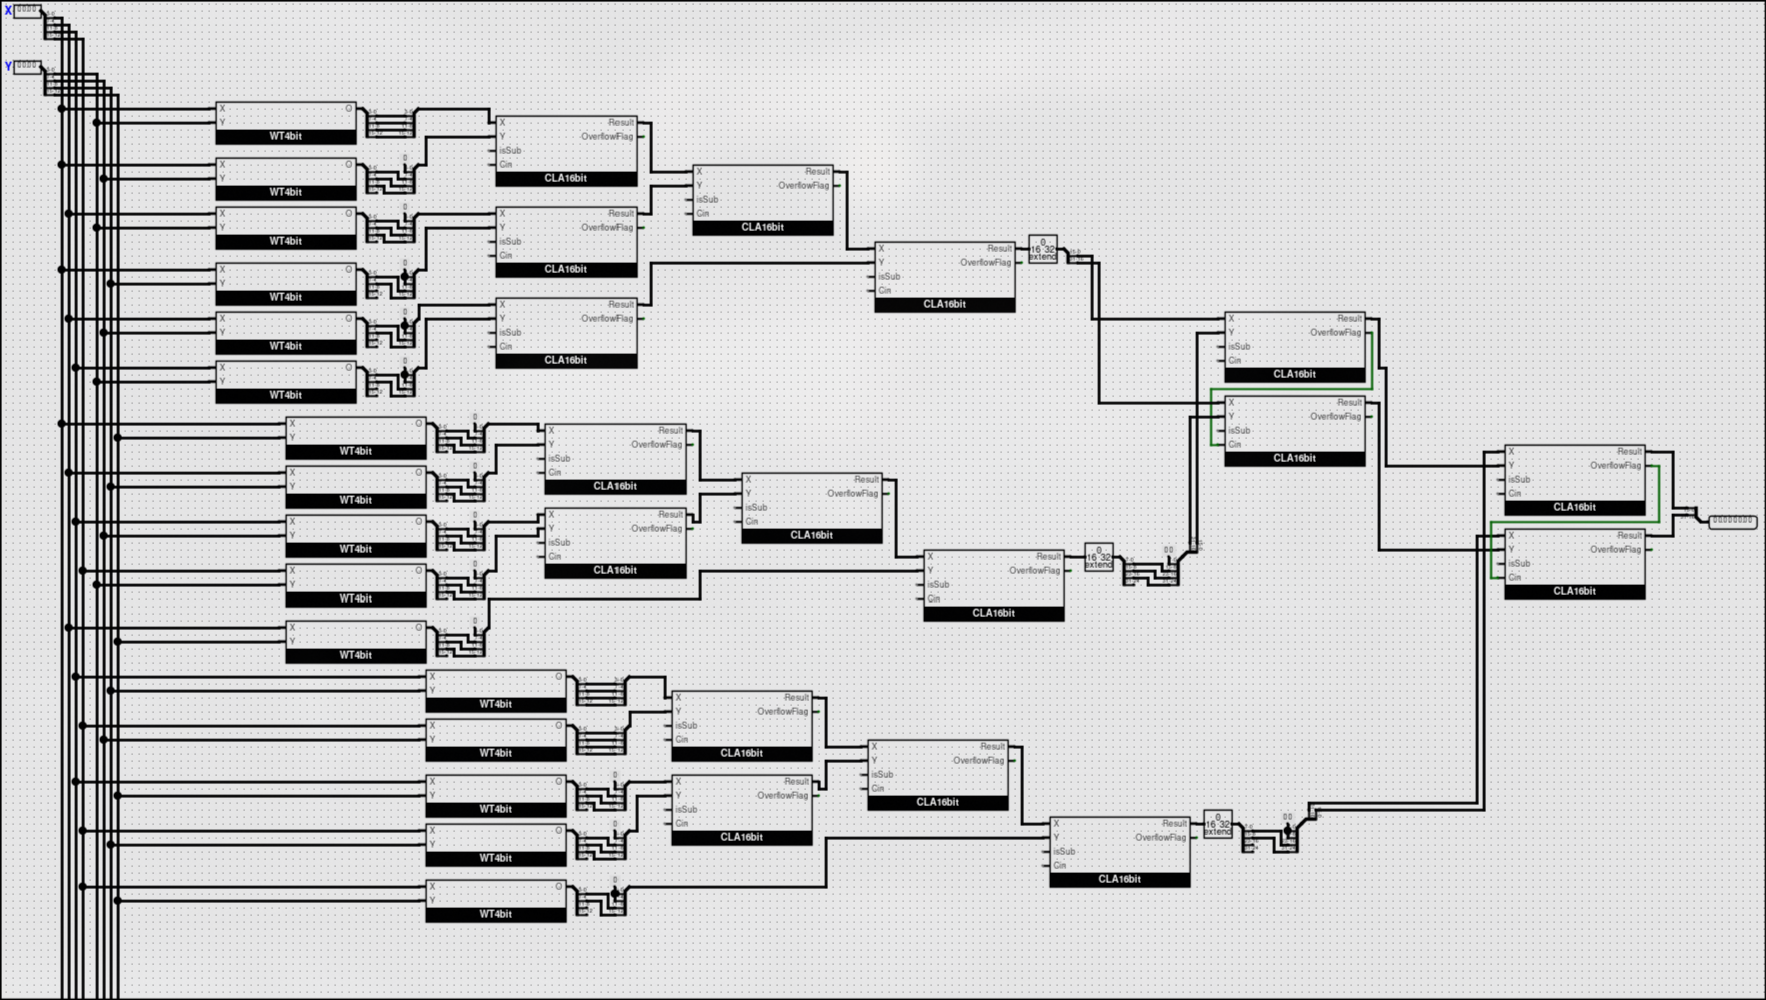
\includegraphics[width=\textwidth]{WT16.png}
        \caption{Full 16-bit Wallace tree looks pretty evil}
        \label{fig:wt16}
    \end{subfigure}
    \caption{4-bit Wallace Tree next to the full 16-bit one}
    \label{fig:wallace_tree_comparison}
\end{figure}

\subsection{GPRs}
GPRs (General-Purpose Registers) are implemented using master-slave D flip-flops utilizing AND and NOR gates, totaling 8 GPRs. One register can be written to, and two registers can be read; reading is implemented using an 8-to-1 MUX. 

\begin{figure}[H]
    \centering
    \begin{subfigure}[b]{0.4\textwidth}
        \centering
        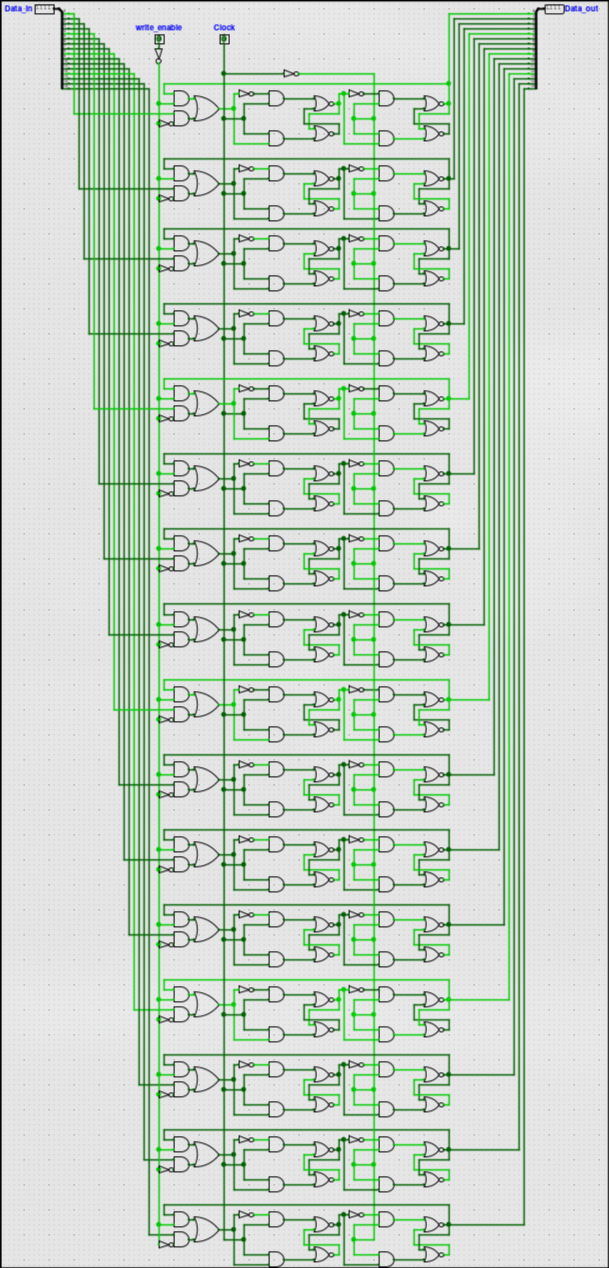
\includegraphics[height=0.5\textheight, keepaspectratio]{Reg16.png}
        \caption{1 16-bit register storing 0x1111}
        \label{fig:reg16}
    \end{subfigure}
    \hfill
    \begin{subfigure}[b]{0.48\textwidth}
        \centering
        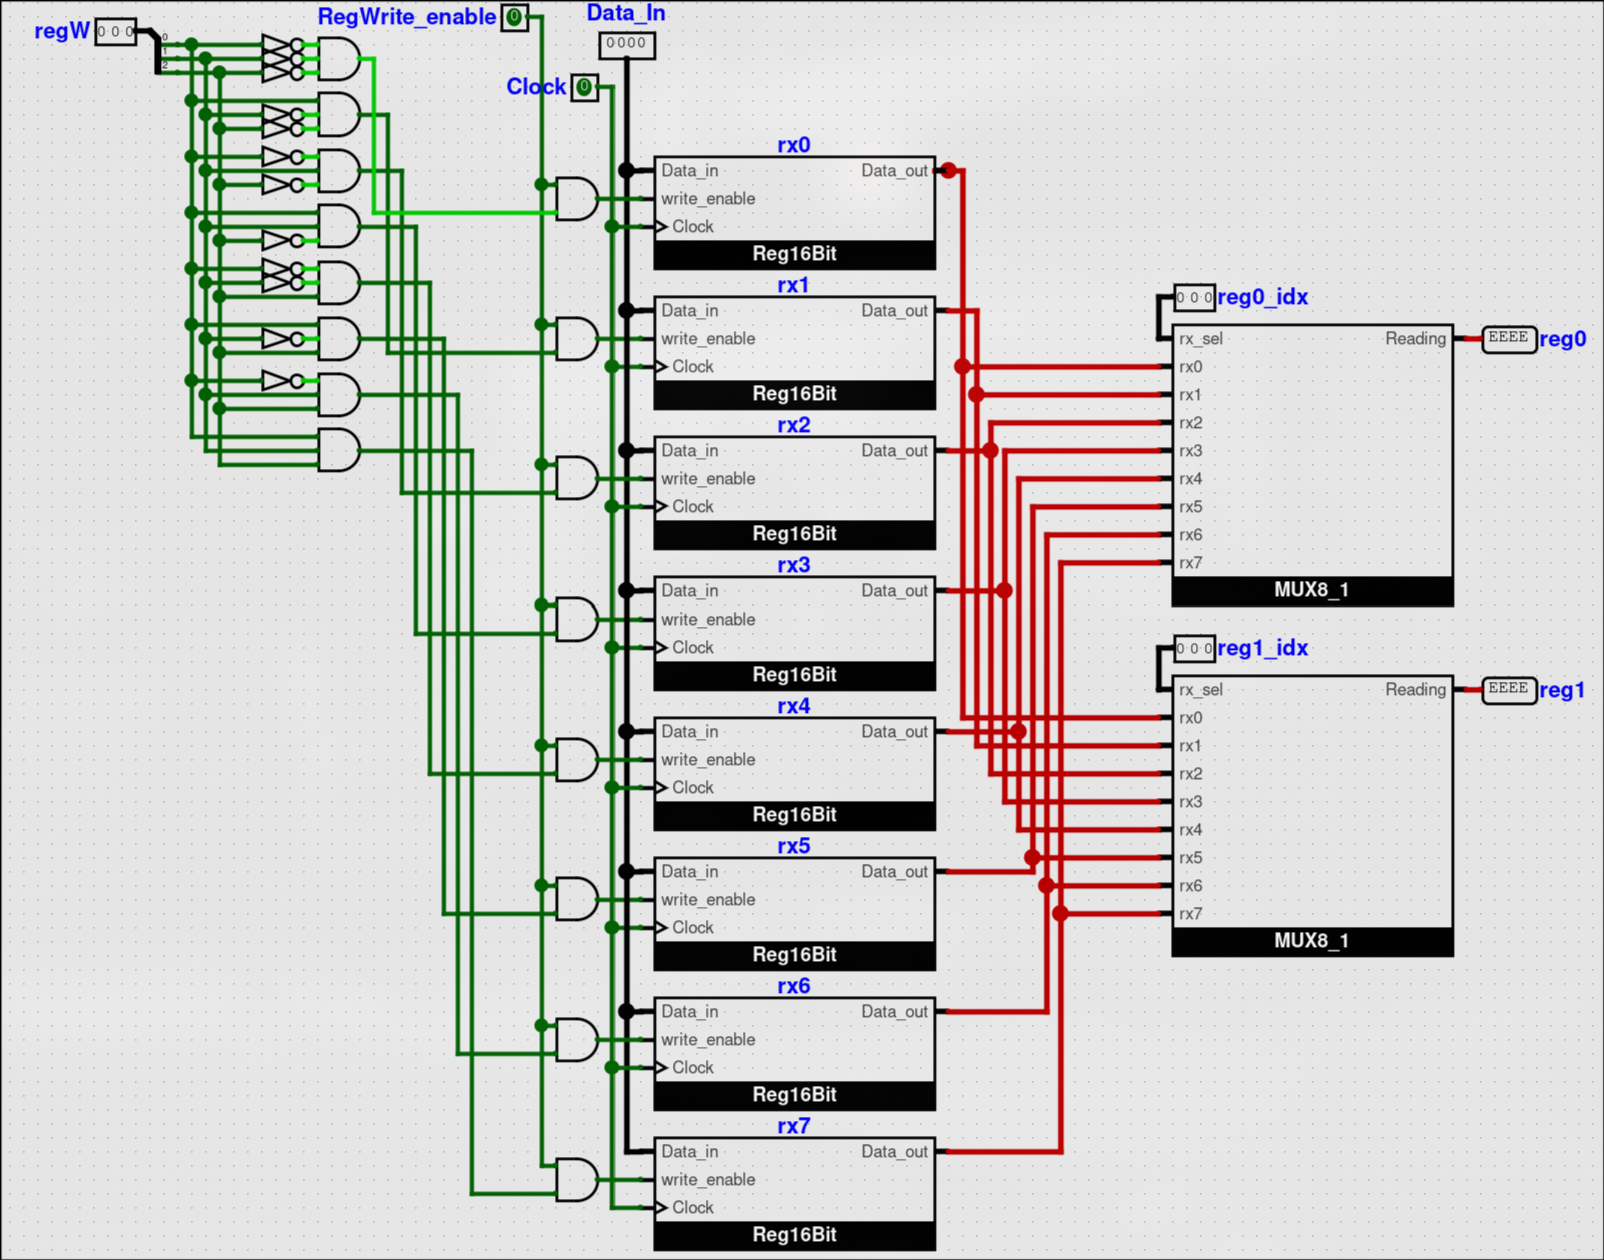
\includegraphics[width=\textwidth]{GPRs.png}
        \caption{Full 8-GPR Register File}
        \label{fig:gpr_file}
    \end{subfigure}
    \caption{All GPRs}
    \label{fig:gpr_comparison}
\end{figure}

\subsection{CU}
The CU (Control Unit) is a finite state machine operating in 6 distinct states. A multi-cycle design was chosen over a single-cycle one because it reduces the critical path length, vastly increasing the maximum possible clock speed. 

\begin{itemize}
    \item \textbf{State 0 (Fetch):} Loads an instruction into the Instruction Register (IR) and increments the Program Counter (PC) register.
    \item \textbf{State 1 (Decode):} Decodes the instruction and acts as a safety state.
    \item \textbf{State 2-5 (Execute-Writeback-Store-Read):} Based on the opcode, calculates particular control signals such as PCWrite for branching, regMux, RAM Read/Write, etc. Resets to State 0 after the instruction has finished, resetting at a different state depending on the instruction type.
\end{itemize}

\begin{figure}[H]
    \centering
    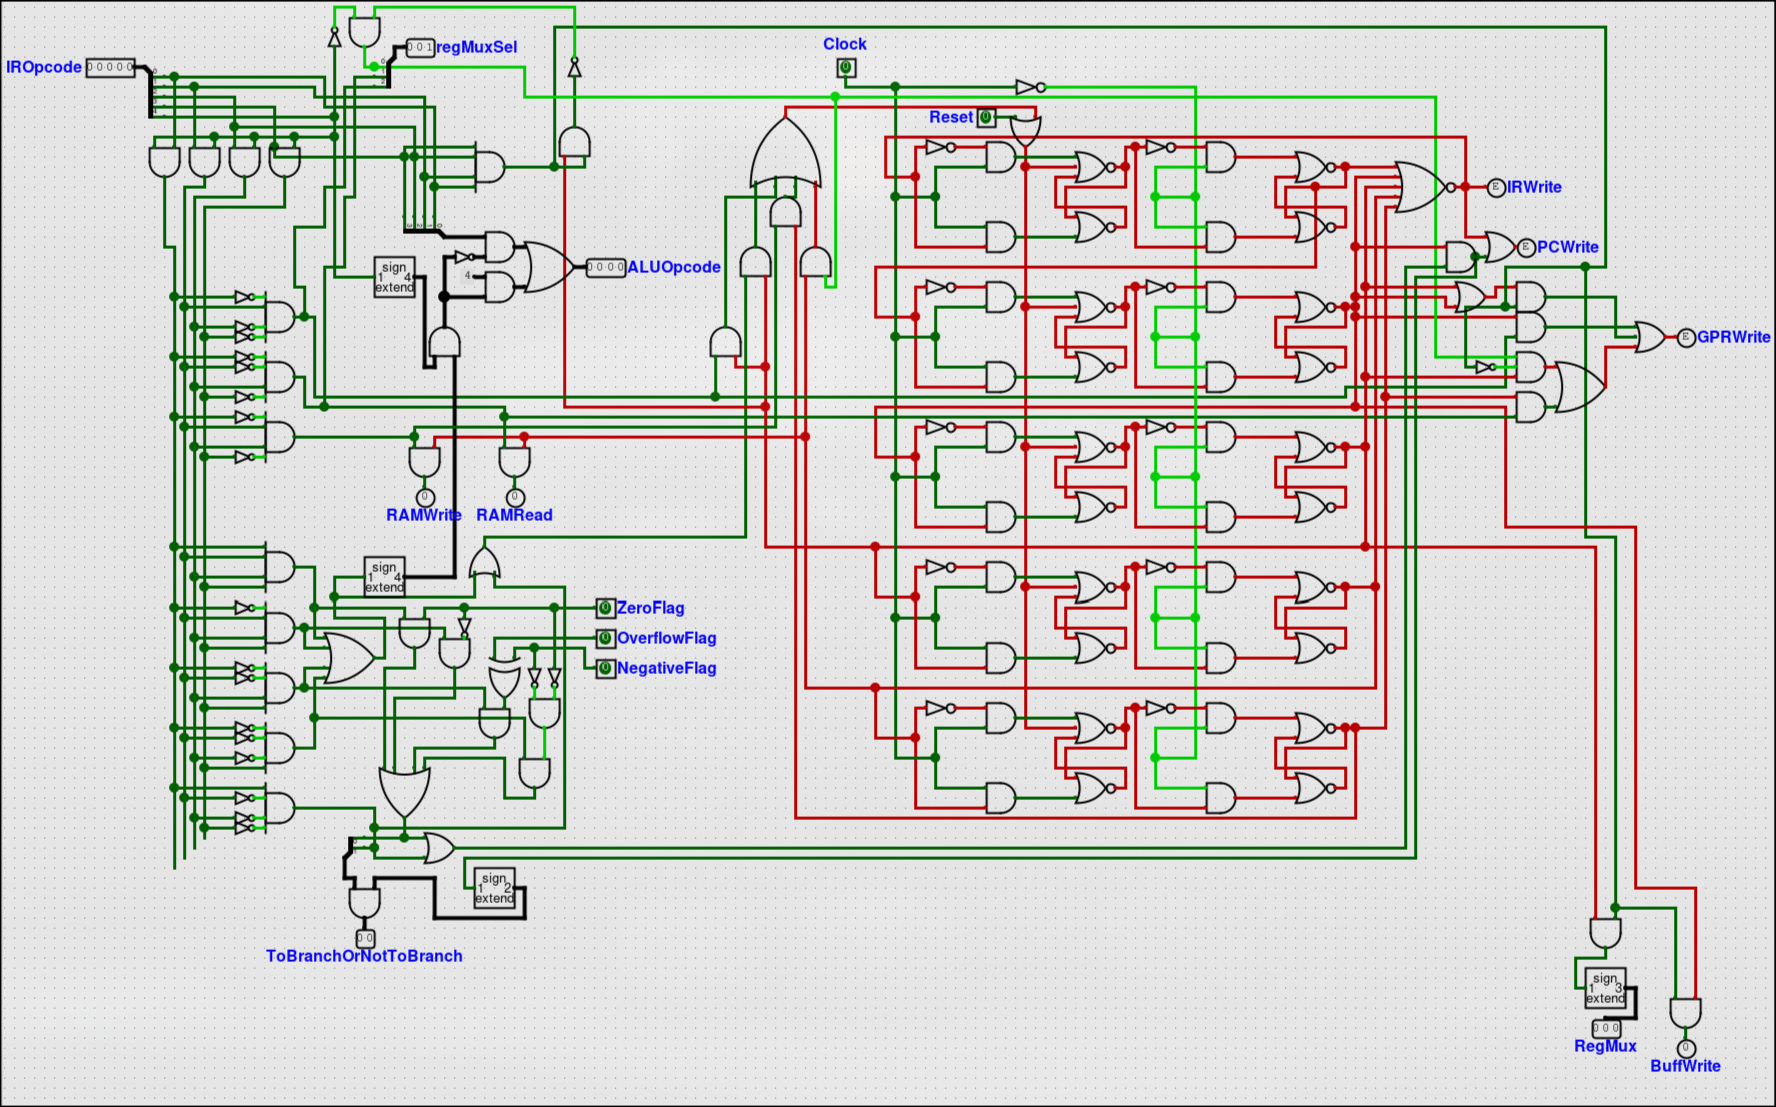
\includegraphics[width=0.55\textwidth]{CU.png}
    \caption{Diagram of the CU}
    \label{fig:cu_diagram}
\end{figure}

\section{Eclipse-100000}
One more 0 indicates 32 bits. This is an actual CPU written in SystemVerilog. This CPU is multi-cycle as well. 

\subsection{Overview}
Eclipse-100000 is a CPU with a completely custom architecture and ISA. The design is lightweight and optimized, focusing on native CPU operating-system support. Its main features are:
\begin{itemize}
    \item 32 32-bit GPRs ($R_X0 - R_X31$) as well as a set of Special-Purpose Registers (SPRs)
    \item Dual-Privileged execution mode implemented using banking of some SPRs
    \item Memory Protection Unit with real-time memory access checks; invalid memory access leads to an immediate jump to the dedicated \texttt{MemoryFault} vector (0x70)
    \item Memory Topology (MMIO) for main memory, VRAM, and I/O
    \item Hardware Interrupt execution every set number of clock cycles that jumps to 0x64 for multitasking, alongside an integrated syscall vector at 0x64
\end{itemize}

\subsection{ISA}
The complete specification is available in \texttt{ISA32.txt}; at the same time, its core features are briefly outlined below. Instructions are 32-bit, encoded using various instruction types. The first 6 bits are always the opcode; subsequent bits depend on the exact type. I refer to the first register in the instruction as \texttt{rx0}, the second as \texttt{rx1}, and the third as \texttt{rx2}. \texttt{Imm} stands for immediate, and the number after it is the bit size specified (e.g., \texttt{imm10} is a 10-bit immediate).

\begin{table}[h!]
\centering
\caption{Eclipse-100000 Instruction Formats}
\label{tab:instruction_types}
\resizebox{\textwidth}{!}{%
\begin{tabular}{|l|l|l|}
\hline
\textbf{Format} & \textbf{Bit Layout} & \textbf{Description / Use Case} \\ \hline
\textbf{R-Type} & Opcode[31:26] | rx0[25:18] | rx1[17:10] | Imm10[9:0] & Standard 2-operand ALU logic/shifts (10-bit unsigned imm) \\ \hline
\textbf{B-Type} & Opcode[31:26] | rx0[25:18] | rx1[17:10] | rx3[9:2] | imm2[1:0] & 3-operand ALU operations with 2-bit loop modifier \\ \hline
\textbf{I-Type} & Opcode[31:26] | rx0[25:18] | rx1[17:10] | Imm10[9:0] & Memory load/store (\texttt{LDR}/\texttt{STR}) with 10-bit signed offset \\ \hline
\textbf{S-Type} & Opcode[31:26] | rx0[25:18] | SPR\_Sel[17:16] | Imm16[15:0] & SPR (\texttt{SP}, \texttt{LR}, \texttt{GP}) ops with 16-bit signed immediate \\ \hline
\textbf{L-Type} & Opcode[31:26] | rx0[25:18] | Imm18[17:0] & Direct load (\texttt{LOAD}) \& stack (\texttt{PUSH}/\texttt{POP}) (18-bit signed imm) \\ \hline
\textbf{J-Type} & Opcode[31:26] | Imm26[25:0] & Jumps (\texttt{JMP}, \texttt{CALL}) \& massive load (\texttt{LMA}) (26-bit imm) \\ \hline
\end{tabular}%
}
\end{table}

\noindent \textbf{Notes:}
\begin{itemize}
    \item \textbf{B-Type:} 2-bit loop modifier made specifically for \texttt{for} loops; it can be -1, +1, or +2 because I hardcoded \texttt{0b10} to be +2 instead of -2, specifically because I consider a +2 loop increment more useful than -2. 
    \item \textbf{S-Type:} Currently 3 SPRs are accessible by the program: Stack Pointer (\texttt{SP}), Link Register (\texttt{LR}) for function return addresses, and General Pointer (\texttt{GP}) used to store initial \texttt{SP} location for globals (more on that in the FLARE-10K section). 
\end{itemize}

\subsection{Register Fragmentation}
A central feature of the architecture is its hierarchical register fragmentation model, which directly simplifies code generation and type casting.

\begin{figure}[H]
    \centering
    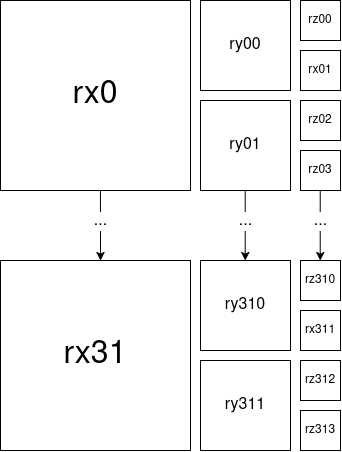
\includegraphics[height=0.5\textwidth]{Fragmented.png}
    \caption{Representation of the principle of Fragmented Registers}
    \label{fig:reg_frag}
\end{figure}

Each 32-bit register ($R_X$) is fragmented into two 16-bit sub-registers ($R_Y$), each of which is further fragmented into two 8-bit ($R_Z$) sub-registers. The last digit in the name represents the sub-register specified, and all preceding digits represent the base register. For example, $R_X16$ is fragmented into $R_Y16[0\text{--}1]$ and $R_Z16[0\text{--}3]$; thus, the highest 8 bits of $R_X16$ would be $R_Z163$. Bear in mind, though, that they are not separate registers but rather parts of one full register, so modifying a sub-register directly modifies its parent register. 

\subsection{Control Unit}
Eclipse-100000 has a total of 10 Finite State Machine states: 
\begin{verbatim}
typedef enum logic [3:0] {
        FETCH,
        DECODE,
        ALU_EXE,
        BRANCH,
        LOAD,
        READ_DATA,
        EXCEPTION,
        TIMER_INTERRUPT,
        MEM_FAULT,
        STORE
} fsm_states;
\end{verbatim}

\begin{figure}[H]
    \centering
    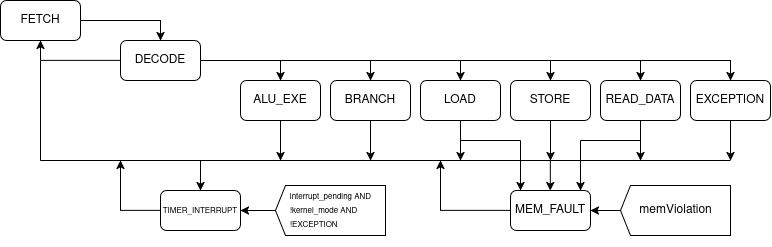
\includegraphics[width=0.55\textwidth]{states.png}
    \caption{Flowchart of the CPU's FSM; squared arrows represent conditions}
    \label{fig:fsm_flowchart}
\end{figure}

\begin{itemize}
    \item \textbf{FETCH:} Fetches the instruction and increments PC by 4 because memory uses byte addressing, so each instruction is 4 bytes.
    \item \textbf{DECODE:} Deduces the next state based on opcode and calculates the effective address ($\text{PC} + \text{RegX}$) since the ALU is idle. Control flow instructions (\texttt{CALL}, \texttt{RET}, \texttt{JR}, \texttt{JMP}) execute during the decode phase to save clock cycles and increase performance.
    \item \textbf{ALU-EXE:} The ALU performs calculations and writes the result back.
    \item \textbf{BRANCH:} Computes whether the branch condition is met or not; if yes, it branches.
    \item \textbf{LOAD:} Loads from memory based on whether it is an SPR read or a regular memory read.
    \item \textbf{READ-DATA:} Reads data from memory; also used for \texttt{POP}.
    \item \textbf{EXCEPTION:} Raises privileges to kernel mode and saves current PC to the respective vector.
    \item \textbf{TIMER-INTERRUPT:} Interrupt that happens every set amount of cycles; raises privileges to kernel mode and saves current PC to the respective vector.
    \item \textbf{MEM-FAULT:} Immediately disables memory access, raises privileges, saves PC, and jumps to the respective vector.
    \item \textbf{STORE:} Stores data in memory; also used for \texttt{PUSH}.
\end{itemize}

\section{FLARE-10K}
FLARE-10K is a statically and strongly typed, AOT-compiled imperative systems language. It is designed to write an OS on; it is generally a C-like language, but considerably different. The documentation is in the \texttt{docs/flare.md} file; therefore, this chapter will focus on explaining implementation specifics. I encourage readers to review the documentation (\texttt{docs/flare.md}) first. The following sections will outline and explain each part of the compiler.

\subsection{Lexical Analysis}
The lexer is the first part of the compiler pipeline. It works by looking at the current character and occasionally peeking at the next one to determine the type of Token it is looking at. 

There is one unique feature of the Lexer: inline Lexing. Inlines are lexed just as they are; however, due to the rather large number of Tokens an inline statement requires, all necessary tokens are pushed to a queue in their respective order, which then get pushed to the final vector of tokens.

\subsection{Parser}
The parser is Recursive Descent LL(1) with localized LL(2) fragments. The parser generates a full Abstract Syntax Tree (AST). The precedence table for my language's grammar is presented below; I took the idea from the book \textit{Crafting Interpreters} by Robert Nystrom. Each block represents a grammar construct; the height represents precedence, meaning higher blocks at some point descend to lower blocks. It is LL(2) for struct/regarch declarations because they consist of an identifier followed by another identifier, though this could have been implemented without using LL(2).

\begin{figure}[H]
    \centering
    
\includegraphics[width=0.55\textwidth]{PrecedenceTable.png}
    \caption{Precedence Table of FLARE-10K}
    \label{fig:precedence_table}
\end{figure}

I believe the precedence table is comprehensive enough to explain the main pipeline of the parser.

\subsection{Semantic Analysis}
The semantic analyzer is rather minimal; however, it still performs basic functions. It iterates through the AST generated by the parser and inserts variables, functions, structs, globals, scopes, loop depths, and the current return name into the general Semantic Struct. It then looks for uninitialized variables, unidentified structs, wrong parameter counts, and other issues. It might misbehave occasionally, but generally, it is a good tool to ensure the program is valid.

\subsection{Intermediate Representation (IR)}
As I mentioned in the documentation, the IR was specifically made fairly general for two main purposes:
\begin{enumerate}
    \item A possible backend for other architectures, and
    \item Preparing for later optimization.
\end{enumerate}

The IR lowers (I prefer the term reduces, or even better, flattens, but I will stick to the official term) the Abstract Syntax Tree into Three-Address Code (TAC).

\subsubsection{IROperand}
An \texttt{IROperand} is literally an operand of an \texttt{IRInst}. There are several \texttt{IROperand} types:
\begin{itemize}
    \item Signed/unsigned constants – Just scalar values like 10.
    \item \texttt{Var} – User-declared variable.
    \item \texttt{Temp} – Value generated by the compiler.
\end{itemize}

\texttt{IROperand}s do not get registers assigned at this point; the IR just specifies that they are registers by either using a variable name or allocating one of infinitely many virtual registers to them (which is often done for constants). Codegen then allocates actual hardware registers to them. This is similar to other \texttt{IROperand}s: they do not actually get memory offsets; the IR just determines in what kind of memory they live, and codegen then handles offsets and everything else.

\subsubsection{lvalue/rvalue Duality}
Depending on the expression type, it gets parsed differently. In one scenario, it gets parsed using a reduce-expression function that produces a value; in another case, by a lower-lvalue function that produces an address. It is used for getting the address of constructs such as structs, arrays, dereferences, and others. 

However, it is worth mentioning that since regarches literally do not have an address, they are parsed as \texttt{RefFieldRead} and \texttt{RegFieldWrite}, which determine what part of the regarch we are accessing and, based on that, output the sub-register we are dealing with (fragmented registers come into play again).

\subsubsection{Functions}
Actually, the IR does work with actual registers in the calling stage: it puts arguments in the first 4 registers, meaning there might be up to 16 arguments passed via these 4 registers assuming they are all 8 bits, like \texttt{u8} or \texttt{bool}. Regarches are placed into one of the 4 input registers; if the first 4 registers are already filled, though, regarches get spilled onto the stack like regular arches or any other variable. As for regular structs and arrays, their addresses get pushed onto the stack, defaulting to pass-by-reference.

Now, return variables are actually pretty simple since they are similar to arguments; they are implemented in a similar way, but with \texttt{NULL} initialization and optional pinning. Also, I used the principle of a void-return function (which by default returns nothing) and applied it to functions with return variables.

\subsubsection{Notes}
Regarding \texttt{AntiEqual}, \texttt{Equal}, etc. naming: for example, \texttt{Less} becomes \texttt{AntiLess}, which in codegen becomes "greater than."

\subsection{Code Generation}
Now, code generation is the most complicated part of FLARE-10K, so I am going to outline its main features at a high level.

\subsubsection{Register Allocation}
To map an unlimited number of virtual registers generated by the IR onto real hardware registers, I use the Chaitin-Briggs optimistic graph-coloring algorithm.

\paragraph{1. Liveness analysis \& interference graph}
The first step is analyzing a variable's liveness. A variable is live at any point in the program if it is going to be read before it gets overwritten (killed) or the program ends. I scan each basic block (the largest sequence of code without branching) from bottom to top - because variables are typically read on the right-hand side of an expression - and determine which variables are live simultaneously.

Afterward, we use the collected data to construct an interference graph where nodes represent a variable's live range, and an edge between nodes indicates that variables are live at the same time.

\paragraph{2. Node removal and spilling}
The next step is to repeatedly remove any node with a degree less than $K$, where $K$, in my architecture, is the register capacity in bytes (120 bytes). Because such nodes have fewer neighbors than available register bytes, they are mathematically and logically guaranteed to get a register. Fortunately, removing any node results in the degree of all neighbors being decreased by 1, thereby simplifying the process. Removed nodes get pushed onto the stack.

However, the algorithm might stall, meaning there are no nodes with a degree $< K$. In that case, a spill weight for each node is computed based on its usage frequency and presence in a loop (if a variable is read in a loop, $10^{\text{loop depth}}$ is added to its spill weight). Then, the node with the lowest spill weight gets optimistically pushed because it is less critical and will decrease the degree of all neighboring nodes, thereby increasing the chances of more important variables being allocated.

\paragraph{3. Coloring}
Finally, variables are popped off the allocation stack one by one to assign physical fragmented registers to them. 16-bit variables are aligned to fit full $R_Y$ registers (in either the lower or higher 16 bits of a register). In most cases, a variable will get allocated - even if it was optimistically pushed - because neighbors often share the same register. However, in rare cases where that does not happen, the last resort comes into play and variables get spilled to the stack.

\paragraph{4. Spill Rewriting and Re-allocation}
Spilled variables rewrite the IR: every time they are read, we load them into a register, and every time they are written, they are stored to memory. Therefore, this changes liveness and it has to be recomputed. This loop happens up to 100 times as a safety valve. 

There is much more to this algorithm. If you are interested, I encourage you to explore it further or read my implementation in the \texttt{codegen.rs} file, where I tried commenting it as comprehensively as possible.

I also want to mention that pinned variables and regarches skip the allocation process, and their assigned registers are marked as used. Also, registers get allocated from the top down (from \texttt{rx29} down) to minimize interference with argument passing.

\subsubsection{Temporary Registers}
Unfortunately, I had to reserve \texttt{rx31} and \texttt{rx30} as temporary registers for code generation because we need a place to store hardcoded constants. Immediately after usage, those registers are XORed with themselves so they become 0, unless the next instruction overwrites them (\texttt{LOAD}/\texttt{LMA}) - a small optimization that really matters in array initialization. 

\subsubsection{Casting}
Casting is very convenient - it heavily utilizes register fragmentation, so a simple \texttt{MOV} instruction is enough for most cases. Moving to larger registers automatically zero-extends/upcasts, while moving to smaller registers automatically truncates to the lower bits. There is one special case: signed upcasting requires an initial \texttt{SHL} followed by an \texttt{SRA}. 

\subsubsection{Globals}
Global variables or structs are stored at a positive \texttt{SP} offset. This works by first calculating the total size of all globals, decreasing the stack pointer by that amount, and then setting the General Pointer SPR (\texttt{GP}) to the current \texttt{SP}. Thus, globals live just before the main stack of the program at a positive \texttt{GP} offset. Global arrays are also supported; they work like regular global variables, loading elements sequentially at positive \texttt{GP} offsets. 

\subsubsection{Branching}
Due to the lack of "jump if less than or equal" (or its counterpart), $\le$ and $\ge$ operations compile down to two instructions: a branch if less/greater, followed by a branch if equal. Fortunately, branching takes only 2 CPU cycles on my architecture, making this a negligible factor in execution speed while saving opcode space for other ISA instructions. 

\subsubsection{Non-Leaf Functions}
A function is non-leaf if it calls another function. This distinction is important because there is only one Link Register (\texttt{LR}), which can store only one return address. Therefore, \texttt{LR} must be saved before calling another function within a non-leaf function; this is resolved by simply pushing it onto the stack right before the call and popping it right after.

\subsubsection{Call Saves}
During a function call, not every variable or register gets spilled to the stack - only live ones do. This is implemented by walking through the basic block containing the call in reverse and using the same mechanism used for liveness analysis to compute which values need to be saved and subsequently restored.

\subsubsection{Stack Argument Resolution}
Arguments that don't fit into the first four argument registers are pushed immediately before \texttt{CALL} by the caller function. On the callee's function side, these are not addressed relative to the incoming stack pointer directly; instead, each is represented in the IR as an \texttt{IncomingArgSlot(idx)}, which codegen lowers to \texttt{SP + local\_frame\_size + idx} $\times$ \texttt{4} once the callee's own prologue has finished decreasing stack for its own spills. This offset has to be computed after \texttt{local\_frame\_size} is known, since every byte the callee reserves for its own frame pushes the caller's pushed arguments further away from \texttt{SP}.

\subsection{Trade-offs}
There are currently several limitations of the compiler that I am planning to fix:
\begin{enumerate}
    \item No multi-expression \texttt{if} statements (\texttt{\&\&} and \texttt{||} are not implemented yet). This is easily worked around by nesting loops and utilizing \texttt{else if} statements.
    \item no callee-saved registers exist at all - everything is caller-saved, though I would hardy call it a trade-off, its just a design decision
    \item Global array's elements must be known literals at compile time
    \item No compile time global evaluation, for example $\#$def u32 a = 5+10; is not valid.
    \item Currently, there are minimal dedicated optimization passes. (Though register allocation itself yields significant speedups.) There are also other optimizatinos, such as no conditions checking for while [true] loops, or stripping useless xors, which I wouldn't call a "dedicated optimization pass", nontheless they do increase execution speed.
    \item FLARE-10K lacks syntactic sugar such as \texttt{+=} and \texttt{-=}.
    \item Functions cannot return arrays, nor can they accept structs or arrays by value (non-reference).
    \item No hardware division or modulo instructions, as I refuse to add them to the ALU without implementing them using purely primitive logic gates in Logisim first.
    \item The allocator halts after 100 rewrite passes, which usually indicates an allocation bug.
\end{enumerate}

\end{document}
